\section{Presentation de l'architecture}

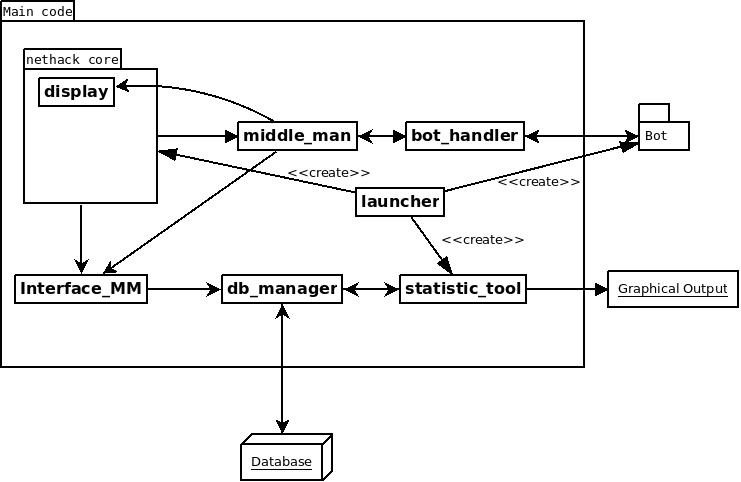
\includegraphics[width=140mm]{Images/new_archi.jpeg}

\begin{description}
\item[Bot Handler: ] Le Bot Handler est la pour traduire le langage haut niveau utilisé par le bot en commande Nethack.
\item[Middle Man: ] le Middle Man communique les instructions Nethack au noyau du jeu et et les messages du jeu au bot via le Bot Handler.
\item[Interface Middle Man: ] L'interface Middle Man transfert les statistiques et les caractéristiques d'une partie dans la base de donnée.
\item[DB Manager :] Le DB Manager est un module contenant les fonctions de manipulation de la base de donnée.
\item[Statistic Tools:] Ce module met en pages les informations contenues dans la base de donnée.  
\end{description}

Une des exigences du client était d'utiliser le langage C pour développer le projet. Nous avons fait le choix de gérer les résultats des parties avec le Système de gestion de base de données Sqlite. Ce choix était motivé par le besoin de stocker potentiellement les resultats de plusieurs milliers de partie et celui de produire des statistiques avec, une base de donnée nous permettant de récuperer les informations de manière très rapide.

Pour l'affichage des statistiques, nous avons développé un module qui génère une page html et du code javascript. Ce choix s'est fait assez naturellement du fait de la souplesse du langage html et des nombreuses bibliothèques javascripts. 
